\documentclass[11pt]{beamer}
\usetheme{JuanLesPins}
\usepackage[utf8]{inputenc}
\usepackage[spanish,es-nodecimaldot]{babel}
\usepackage{amsmath}
\usepackage{amsfonts}
\usepackage{amssymb}
\usepackage{graphicx}
\usepackage{adjustbox}
\usepackage{array}
\spanishdecimal{.}
\author{M. en E. Sergio Nava}
\title{Variable Aleatoria}
%\setbeamercovered{transparent} 
%\setbeamertemplate{navigation symbols}{} 
%\logo{} 
%\institute{} 
\date{Viernes 7 de octubre de 2016} 
%\subject{} 

\AtBeginSection[]  % The commands within the following {} will be executed at the start of each section.
{
\begin{frame} % Within each "frame" there will be one or more "slides."  
\frametitle{Presentation Outline} % This is the title of the outline.
\tableofcontents[currentsection]  % This will display the table of contents and highlight the current section.
\end{frame}
} % Do not include the preceding set of commands if you prefer not to have a recurring outline displayed during your presentation.


\begin{document}

\begin{frame}
\titlepage
\end{frame}



\section{Variable Aleatoria}
\begin{frame}{Variable Aleatoria}
\begin{itemize}
\item La variable \emph{X} se llama variable aleatoria si los valores que toma \emph{corresponden} a los distintos resultados posibles de un determinado experimento, y por ello el hecho de que tome un valor particular es un evento aleatorio.
\item Una Variable Aleatoria (v.a.) es una regla que asocia a los elementos muestrales con valores numéricos.
\end{itemize}
\end{frame}
\begin{frame}{Variable Aleatoria}
\begin{center}
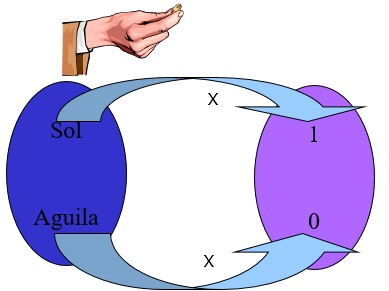
\includegraphics[scale=0.7]{imagenes/prob38.jpg} 
\end{center}
\end{frame}


\section{Variables Aleatorias Discretas y Contínuas}

\begin{frame}{Variable Aleatoria}
\begin{center}
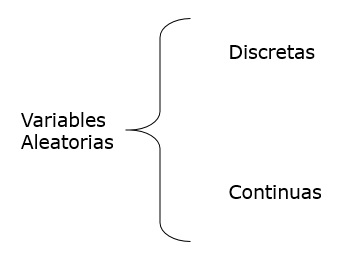
\includegraphics[scale=0.8]{imagenes/prob39.jpg} 
\end{center}
\end{frame}
\begin{frame}{Variable Aleatoria Discreta}
Es aquella que toma, a lo más, una cantidad numerable de valores distintos; Esto quiere decir que estos valores se pueden asociar a los enteros 0, 1, 2, 3, ......., en otras palabras, que se pueden numerar.

\end{frame}
\begin{frame}{Variable Aleatoria Continua}
Es aquella que puede tomar cualquier valor de entre todos los contenidos en un intervalo de la recta. 
	En estos casos comúnmente se utilizan instrumentos de medición. Dependiendo de la exactitud del instrumento utilizado, cada posible valor de $x$ podría, al menos desde el punto de vista teórico, considerarse como un punto en un intervalo de la recta. 

\end{frame}
\begin{frame}{Ejemplos de v.a. discretas}
\begin{small}
\begin{tabular}{|m{10em}|m{8em}|m{8em}|}

\hline
 \emph{Experimento} & \emph{v.a. X} &\emph{Valores posibles} \\ \hline
Llamar a cinco clientes & Cantidad de clientes que han pedido & 0,1,2,3,4,5 \\ \hline
Inspeccionar un embarque de 50 radios & Cantidad de radios defectuosos & 0,1,2,3,...,50 \\ \hline
Funcionamiento de un restaurante durante un dia & Cantidad de clientes & 0,1,2,... \\ \hline
Vender un automovil & Sexo del cliente & 0 si es hombre,1 si es mujer \\ \hline
Inspeccionar artículos de una línea de producción & número de artículos inspeccionados hasta encontrar 5 defectuosos & 5, 6, \ldots \\ \hline
\end{tabular}
\end{small}
\end{frame}
\begin{frame}{Ejemplos de v.a. continuas}
\begin{small}
\begin{tabular}{|m{10em}|m{8em}|m{8em}|}

\hline
 \emph{Experimento} & \emph{v.a. X} &\emph{Valores posibles} \\ \hline
Funcionamiento de un banco & Tiempo en minutos entre llegadas de clientes & $x\geq 0$ \\ \hline
Llenar una lata de bebida (max. 12.1 onzas) & Cantidad de onzas & $0\leq x \leq 12.1$ \\ \hline
Proyecto para construir una nueva biblioteca & Porcentaje de termino de proyecto en seis meses & $0 \leq x \leq 100$ \\ \hline
Ensayar un nuevo proceso quimico & Temperatura cuando se lleve a cabo la reaccion deseada (min 150 $^oF$; max 212 $^oF$) & $150 \leq x \leq 212$  \\ \hline

\end{tabular}
\end{small}
\end{frame}


\section{Distribuciones de Probabilidad y Función de Distribución}
\begin{frame}{Distribución de probabilidad de v.a. discretas}
\begin{itemize}
\item Una variable aleatoria discreta $X$ representa los resultados de un espacio muestral, y $P(X=x)$ representa la probabilidad de que la variable $X$ tome el valor de $x$. 
\item Se llamará a $p(x) \equiv P(X=x)$ \textbf{función de probabilidad} de una variable aleatoria $X$, si satisface que: 
\begin{enumerate}
\item $p(x) \geq 0$ para todos los valores x de X.
\item $$\sum_{x}p(x) = 1$$
\end{enumerate}
\end{itemize}
\end{frame}
\begin{frame}{Función de Distribución Acumulada de v.a. discretas}
La función de distribución acumulada de la variable aleatoria X es la probabilidad de que X sea menor o igual a un valor específico x, esta dada por:

$$F(x)\equiv P(X\leq x)=\sum_{x_i \leq x}p(x_{i})$$
\end{frame}
\begin{frame}{Función de Distribución Acumulada}
Una función F(x) es una función de distribución si y sólo si cumple las siguientes condiciones:
\begin{itemize}
\item $\lim_{x\longrightarrow-\infty}F(x)=0$ y $\lim_{x\longrightarrow-\infty}F(x)=1  $ 
\item F(x) es una funcion no decreciente
\item F(x) es continua por la derecha:
\begin{center}
$\forall h> 0,\lim_{h\rightarrow-\infty}F(x+h)=F(x) $
\end{center}
\end{itemize}
\end{frame}
\begin{frame}{Función de Probabilidad y de Distribución Acumulada.}
\begin{center}
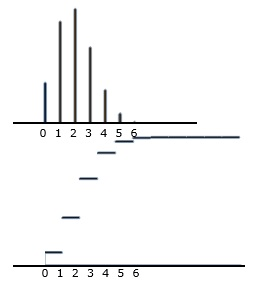
\includegraphics[scale=0.8]{imagenes/prob40.jpg} 
\end{center}
\end{frame}
\begin{frame}{Ejemplo de v.a. discreta}
Consideremos el ejemplo de tirar un dado, y definamos a $X$, la variable aleatoria, como el número en la cara superior. Hay $n=6$ valores posibles de la variable aleatoria, son $ x=1, 2, 3, 4, 5, 6 $ por consiguiente, la función de probabilidad para esta variable aleatoria es 
\begin{center}
 $P(x)=1/6$ \hspace{20pt}  $x=1,2,3,4,5,6$ \hspace{20pt}  $F(x)= \lfloor x \rfloor /6$
 \end{center} 
\begin{center}
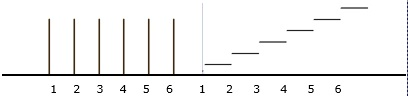
\includegraphics[scale=0.7]{imagenes/prob41.jpg} 
\end{center}
\end{frame}


\section{Valor Esperado}


\begin{frame}{Valor Esperado o  Esperanza Matemática}
\begin{itemize}
\item El valor esperado de una variable aleatoria esta definida por:
$$E\textit{(X)}=\sum xp(x)$$ si \textit{x} es discreta, y se le denota por: $E(\textit{x})=\mu$
\item En general, el valor esperado de una función \textit{g(x)} de la variable aleatoria X, está dada por:
$$E(\textit{g(x)})=\sum \textit{g(x)p(x)}$$ si $X$ es discreta
\end{itemize}
\end{frame}

\begin{frame}{Propiedades del valor esperado}
\begin{enumerate}
\item El valor esperado de una constante es el valor de la constante
\begin{center}
$E(\textit{c})=\textit{c}$
\end{center}
\item El valor esperado de $aX + b$, en donde $a$ y $b$ son constantes es	
$$E(\textit{a}X+\textit{b})=\textit{a}E(X)+\textit{b}$$
\item El valor esperado de la suma de dos funciones $g(x)$ y $h(x)$ de $X$ es
$$E(\textit{g(x)+h(x)})=E(\textit{g(x)})+E(\textit{h(x)})$$
\end{enumerate}
\end{frame}
\begin{frame}{Ejemplo de cálculo de valor esperado}
\begin{center}
\begin{tabular}{rrr}
\textbf{x}&\textbf{p(x)}&\textbf{xp(x)} \\
0&.\hspace{2cm}18&.\hspace{2cm}0(.18)=0.00 \\
1&.39&1(.39)=0.39 \\
2&.24&2(.24)=0.48 \\
3&.14&3(.14)=0.42 \\
4&.04&4(0.4)=0.16 \\
5&.01&5(0.1)=0.05 \\
& &1.50 \\
\end{tabular} \\
$E(x)=\mu=\sum xp(x)$ 
\end{center}

\end{frame}
\begin{frame}{Ejemplo de cálculo de valor esperado (cont.)}
\begin{center}
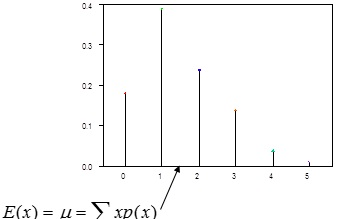
\includegraphics[scale=0.8]{imagenes/prob42.jpg} 
\end{center}

\end{frame}
\begin{frame}{Juego}
El juego es el siguiente, ustedes escogen un número entero del uno al seis, yo tiro tres dados,  si sale 1, 2 o tres veces el número que escogieron, les pago un dólar, y si no sale ni una vez, ustedes me pagan un dólar.\\
\begin{center}
   ¿Cuál es la ganancia o pérdida esperada?
\end{center}
\end{frame}
\begin{frame}{Juego II}
Ustedes escogen un número entero del uno al seis, yo tiro tres dados,  les doy un dólar por cada acierto que logren de los tres dados, y si no aciertan ni un dado, ustedes me pagan un dólar.\\
\begin{center}
   ¿Cuál es la ganancia o pérdida esperada?
\end{center}
\end{frame}


\section{Varianza y Desviación Estándar}

\begin{frame}{Varianza}
La varianza es un promedio ponderado de las desviaciones de una variable aleatoria respecto a su promedio, elevadas al cuadrado. \\
\bigskip
	Los factores de ponderación son las probabilidades.

$$Var(X)=E(X-E(X))^{2}$$
Por lo que la varianza de una variable aleatoria discreta es
$$Var(X)=\sigma^{2}=\sum(x-\mu)^{2}p(x)$$
\end{frame}
\begin{frame}{Varianza}
\begin{itemize}
\item La varianza de cualquier variable aleatoria es no negativa, es decir:
$$Var(X)\geq 0$$
\item La varianza de cualquier variable aleatoria es invariable ante traslaciones; por ejemplo tenemos que:
$$Var(X+b)=Var(X)$$
\item De manera más general, se tiene que:
$$Var(aX+b)=a^{2}Var(X)$$
\end{itemize}
\end{frame}
\begin{frame}{Ejemplo de cálculo de la varianza}
\begin{center}
\begin{tabular}{|r|r|r|r|r|r|}
\hline
\textbf{$x$}&\textbf{$p(x)$}&\textbf{$xp(x)$}&\textbf{$x-\mu$}&$(x-\mu)^{2}$&\textbf{$(x-\mu)^{2}p(x)$}  \\ \hline
0&.18&0.00&-1.5&2.25&0.4050  \\ \hline
1&.39&0.39&-.5&0.25&0.0975  \\ \hline
2&.24&0.48&.5&0.25&0.0600  \\ \hline
3&.14&0.42&1.5&2.25&0.3150  \\ \hline
4&.04&0.16&2.5&6.25&0.2500  \\ \hline
5&.01&0.05&3.5&12.25&0.1225  \\ \hline
&&{\bf 1.50}&&&{\bf 1.2500}  \\ \hline     
\end{tabular}
$E(x)=\mu=\sum xp(x) \hspace{1cm} Var(X)=\sigma^{2}=\sum(x-\mu)^{2}p(x)$
\end{center}
\end{frame}
\begin{frame}{Media y Varianza de una V.A. discreta}
\begin{center}
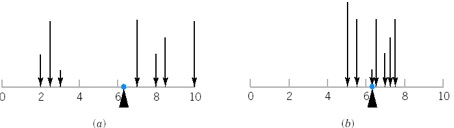
\includegraphics[scale=0.8]{imagenes/prob44.jpg} 
\end{center}
Las gráficas (a) y (b) ilustran las mismas medias, pero (a) tiene una varianza más grande.

\end{frame}
\begin{frame}{Media y Varianza de una V.A. discreta}
\begin{center}
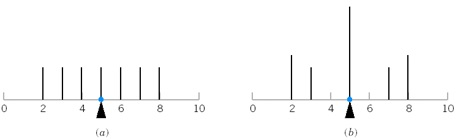
\includegraphics[scale=0.8]{imagenes/prob45.jpg} 
\end{center}
La distribución de probabilidad ilustradas en (a) y (b) son diferentes aun cuando tienen la misma media y varianza.

\end{frame}\end{document}

